Nesta seção, será definido os principais elementos de Market Making.

Um agente pode enviar uma ordem limite $o = (p, Q)$, onde $p$ é o valor da ordem e $Q$ é a quantidade ofertada. Para um intervalo de tempo $t < T$, é possível ter um conjunto de ordens enviadas pelo agente $o_{t} \in \{o_{0}, ..., o_{T}\} = O$ indexados pelo índice de tempo $t$.

A diferença entre o preço da melhor oferta de compra e venda no livro para um determinado ativo é chamada de \textit{bid-ask spread}: $\Delta = p^{(a, 0)} - p^{(b, 0)}$, onde $p^{(a, 0)}$ é o melhor $ask$ e $p^{(b, 0)}$ é o melhor \textit{bid}. Para um \textit{bid} (ou \textit{ask}) em uma posição qualquer, denota-se $p^{(b, i)}$, onde $i$ é a posição no livro de ofertas (decrescente para \textit{bids} e crescente para \textit{asks})

O objetivo de uma estratégia de \textit{market making} (\textit{MM}) nesse contexto é criar ofertas de compra com valor maior (ou menor para ofertas de venda) que venham a se tornar as melhores ofertas, tais que: 

\begin{itemize}
    \item $p^{(a, 0)} < p^{(a, MM)}$ para vendas;
    \item $p^{(b, 0)} > p^{(b, MM)}$ para compras;
\end{itemize}

onde $p^{(MM)}$ é o preço da oferta do agente e  $p^{(0)}$ é a melhor oferta existente.
É importante notar que quaisquer ordens criadas por um agente de \textit{MM} não geram novas transações no momento, ou seja, as ofertas de bid do agente não cruzam com ofertas de ask existentes e vice-versa. ($p^{(a, 0)} > p^{(b, MM)}$ e $p^{(b, 0)} < p^{(a, MM)}$ para novas ordens).

\begin{figure}[H]
	\begin{center}
		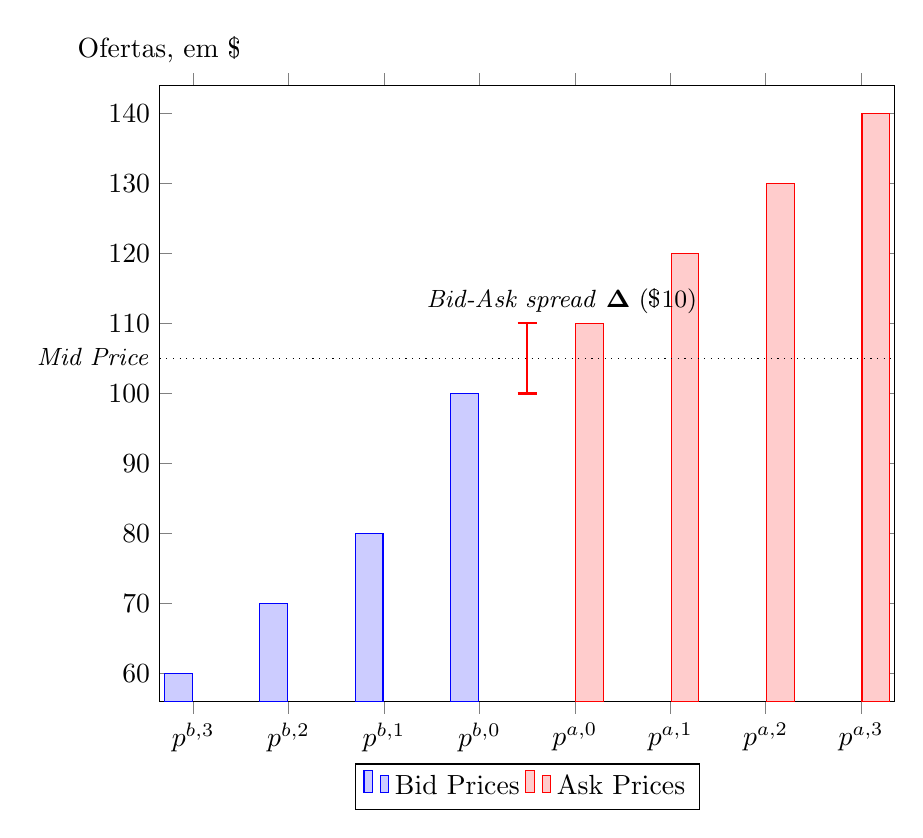
\begin{tikzpicture}
			\begin{axis}[
				x tick label style={/pgf/number format/1000 sep=},
				enlargelimits=0.05,
				legend style={at={(0.5,-0.1)}, anchor=north,legend columns=-1},
				ybar=0.7,
				ylabel={Ofertas, em \$},
    				ylabel style={
    				at={(0,1.02)},
    				anchor=south,
    				rotate=-90,
    			},
				width=0.9\textwidth, % Adjust the width to fit within the box
				xticklabels={
					$p^{b, 3}$, $p^{b, 2}$, $p^{b, 1}$, $p^{b, 0}$, 
					$p^{a, 0}$, $p^{a, 1}$, $p^{a, 2}$, $p^{a, 3}$
					},
				xtick={1,2,3,4,5,6,7,8}, % Set explicit tick positions
				after end axis/.code={
					\draw [red, thick, line cap=] (axis cs:4.5,100) -- (axis cs:4.5,110); % Static vertical line for spread with end caps
					\draw [red, thick] (axis cs:4.4,100) -- (axis cs:4.6,100);
					\draw [red, thick] (axis cs:4.4,110) -- (axis cs:4.6,110);
					\draw [black, dotted] (axis cs:0.65,105) -- (axis cs:8.35,105);
					\node[right, font=\small] at (rel axis cs:0.35,0.65) {\textit{Bid-Ask spread} $\mathbf{\Delta}$ (\$10)}; % Label for the spread line
					\node[left, font=\small] at (rel axis cs:0,0.56) {\textit{Mid Price}};
				}
				]
				% Represent bid prices in blue
				\addplot [blue, fill=blue!20] coordinates {(1, 60) (2, 70) (3, 80) (4, 100)};
				% Represent ask prices in red
				\addplot [red, fill=red!20] coordinates {(5, 110) (6, 120) (7, 130) (8, 140)};
				\legend{Bid Prices, Ask Prices}
			\end{axis}
		\end{tikzpicture}
	\end{center}
	\caption{Gráfico de ofertas de um livro de ordens limite $L$ qualquer}
\end{figure}

\begin{figure}[H]
	\begin{center}
		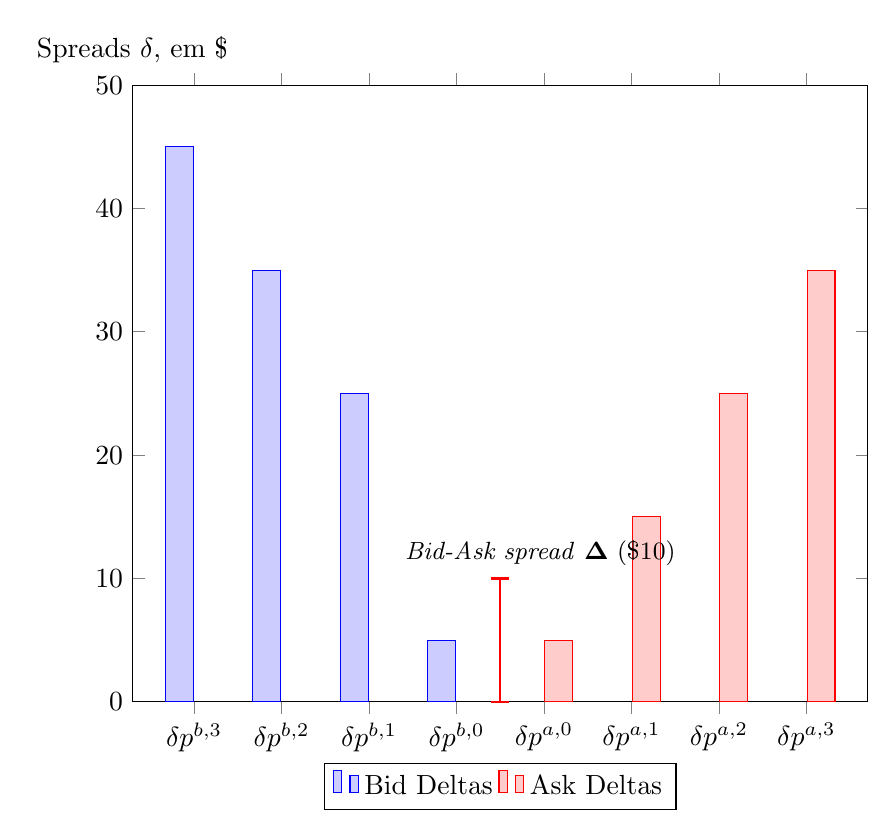
\begin{tikzpicture}
			\begin{axis}[
				x tick label style={/pgf/number format/1000 sep=},
				legend style={at={(0.5,-0.1)}, anchor=north,legend columns=-1},
				ybar=0.7,
				ylabel={Spreads $\delta$, em \$},
				ylabel style={
					at={(0,1.02)},
					anchor=south,
					rotate=-90,
				},
				ymin=0, ymax=50,
				width=0.9\textwidth, % Adjust the width to fit within the box
				xticklabels={
					$\delta p^{b, 3}$, $\delta p^{b, 2}$, $\delta p^{b, 1}$, $\delta p^{b, 0}$, 
					$\delta p^{a, 0}$, $\delta p^{a, 1}$, $\delta p^{a, 2}$, $\delta p^{a, 3}$
					},
				xtick={1,2,3,4,5,6,7,8}, % Set explicit tick positions
				after end axis/.code={
					\draw [red, thick, line cap=] (axis cs:4.5,0) -- (axis cs:4.5,10); 
					% Static vertical line for spread with end caps
					\draw [red, thick] (axis cs:4.4,0) -- (axis cs:4.6,0);
					\draw [red, thick] (axis cs:4.4,10) -- (axis cs:4.6,10);
					\node[right, font=\small] at (axis cs:3.3,12) {\textit{Bid-Ask spread} $\mathbf{\Delta}$ (\$10)}; % Label for the spread line
				}
				]
				% Represent bid prices in blue
				\addplot [blue, fill=blue!20] coordinates {(1, 45) (2, 35) (3, 25) (4, 5)};
				% Represent ask prices in red
				\addplot [red, fill=red!20] coordinates {(5, 5) (6, 15) (7, 25) (8, 35)};
				\legend{Bid Deltas, Ask Deltas}
			\end{axis}
		\end{tikzpicture}
	\end{center}
	\caption{Gráfico de spreads $\Delta$ de um livro de ordens limite $L$ qualquer}
\end{figure}

Para ilustrar melhor o funcionamento do livro de ordens considere a seguinte situação, para um único ativo: um agente qualquer de \textit{MM} tem a \textbf{única oferta de venda} pelo preço de $p^{(a, MM)}$ no mercado. Caso surja uma nova oferta de \textbf{compra} com melhor preço e acima do preço da oferta do agente $p^{(b, i)} \geq p^{(a, MM)}$, será gerada uma transação pelo preço $p^{(a, MM)}$ e a ordem de valor $p^{(b, i)}$ que gerou a transação é a ordem limite com preço de mercado. Após o motor de transações da bolsa receber a oferta $i$, uma transação ocorre e ambas ofertas são removidas do livro de ordens. Em seguida, o agente tem o valor do seu inventário $I$ ajustada:
\begin{equation}
    \begin{aligned}
    	I_{t} = N^{(b)}_{t} - N^{(a)}_{t} 
    \end{aligned}
\end{equation}
onde $I_{t} \in \mathbf{I}, t < T$ é um valor escalar e representa a quantidade que o agente possúi do determinado ativo no momento $t$, e $\mathbf{I}$ é um vetor representado o histórico temporal de inventário do agente. $N^{(a)}$ e $N^{(b)}$ são variáveis aleatórias que representam a quantidade de ativos vendidos ou comprados da oferta inicial, distribuídas de acordo com um processo de contagem, com incrementos indepentes (note que os valores esperados dos incrementos dos processos seguem médias $\lambda_{t}^{(a)}$ e $\lambda_{t}^{(b)}$ que se alteram de acordo com o tempo $t$). Os incrementos dos processos de contagem são limitados externalmente à quantidade ofertada pelo agente, tal que $(N_{t + 1}^{(a)} - N_{t}^{(a)}) \leq Q_{t + 1}^{(a)}$ e $(N_{t + 1}^{(b)} - N_{t}^{(b)}) \leq Q_{t + 1}^{(b)}$.

O retorno financeiro do agente (também chamado de \textit{Profit and Loss} ou \textit{PnL}) é representado por $W$, e também pode ser indexado pelo tempo $W_{t} \in \mathbf{W}, t < T$. O PnL do agente é atualizado de acordo com a seguinte expressão:
\begin{equation}
	\begin{aligned}
		W_{t + 1} = W_{t} + p^{(a, MM)}_{t} \cdot (N^{(a)}_{t + 1} - N^{(a)}_{t}) - p^{(b, MM)}_{t} \cdot (N^{(b)}_{t + 1} - N^{(b)}_{t} )
	\end{aligned}
\end{equation}

Por fim, o agente tem como valor do portfólio a seguinte expressão:

\begin{equation}
	\begin{aligned}
		W_{t} + I_{t} \cdot P_{t}
	\end{aligned}
\end{equation}

onde $P_{t}$ é o preço médio do ativo ($\frac{p_{t}^{(a, 0)} - p_{t}^{(b, 0)}}{2}$) e é distribuido de acordo com um processo de Wiener: $dP_t = \sigma \cdot dz_t$.

A cada observação e atualização dos valores $\{t, P_{t}, W_{t}, I_{t}\}$ o agente pode escolher não fazer nada ou realizar uma das ações abaixo:
\begin{enumerate}
    \item alterar as quantidades ofertadas $Q^{(a)}_{t + 1}$ e $Q^{(b)}_{t + 1}$;
    \item alterar os preços ofertados $p^{(a, MM)}_{t + 1}$ e $p^{(b, MM)}_{t + 1}$;
\end{enumerate}

O agente realiza essas mudanças buscando maximizar a recompensa de sua posição, representada por:

\[
R_{t} =
\begin{cases}
	0 & \text{se } t + 1 < T, \\
	U(W_{t + 1} + I_{t + 1} \cdot P_{t + 1}) & \text{se } t + 1 = T.
\end{cases}
\]

onde U é uma função de utilidade côncava escolhida de forma a levar em consideração o risco associado à posição do agente, tal que $U(x) = -e^{-c x}$ e $c$ é o coeficiente de aversão ao risco.

Em seguida, definimos como $G$ o retorno do agente (agora o termo "retorno" pertence ao contexto de controle estocástico, e não é referente ao "retorno financeiro"), que é a soma amortecida $\gamma$ das recompensas intermediárias:

\begin{equation}
	\begin{aligned}
		G_{T} = \sum_{t=0}^{T} \gamma^t \cdot R_t
	\end{aligned}
\end{equation}

Por fim, o objetivo do agente é obter uma política $\pi$ que maximize a equação ação-valor ótima de Bellman para o tempo terminal (fechamento do pregão) \citep{Sutton2018}.

\begin{equation}
	\begin{aligned}
		Q^{\pi}(s, a) = \mathbb{E}_{\pi} \left[ G_t \mid S_{t} = s, A_{t} = a \right]\\
		Q^{*}(s, a) = \max_{\pi} Q^{\pi}(s, a)		
	\end{aligned}
\end{equation}

Na próxima seção será definido o Processo de Recompensa de Markov, assim como o modelo do ambiente e do agente. Por fim, será discutido o uso de algoritmos de Aprendizado por Reforço para aproximar os valores da equação de Bellman, e da política $\pi$ que maximizem o retorno do agente de \textit{Market Making}.
